\usepackage{graphicx}
\graphicspath{ {./images/} }
\chapter*{Cadrage}

\section*{Finalités et importance du projet}
Comme présenté dans le document d'état de l'art, ce projet vise à présenter une Application Web, disponible sur téléphone, permettant à tout un chacun de: \\
	\textbf{Pour les particuliers} de mettre les fruits/légumes de leur jardin (personnel ou non) à disponibilité de tout un chacun, dans le but de réduire le gaspillage \\
	\textbf{Aux AMAP, circuits courts, producteurs locaux...} de mettre leur production en ligne \\
	\textbf{Aux particuliers} (connsommateurs) d'accéder aux produits en vente\\

Le principal intérêt de la plateforme se voulant d'être unique et intuitids, afin d'être accessible à un maximum d'utilisateurs

\section*{Contexte /Hypothèses de départ}
De nombreuses applications/sites web existent déjà, mais sans contenu "centralisé", mais également afin de pouvoir gérer/visualiser l'entiereté de la chaîne depuis une unique application: ainsi, de nombreuses infrastructures (par exemple les AMAP) ne possèdent pas de service de messagerie spécialisée (dans le cas précédant, la communication se faisant par \textit{mailing-list})\\
Ainsi le produit final devra permettre à l'utilisateur, de manière intuitive, d'accéder à un seul endroit, non seulement d'accéder à la liste des produits disponibles aux alentours (si possible sous forme de carte), mais également d'avoir des nouvelles des agriculteurs, de s'informer des prochaines réunions, de chatter avec tout membre de l'infrastructure...

\section*{Objectifs et résultats opérationnels}
Le but du projet sera de développer les outils suivants:


\newpage

\section*{Organisation./ressources, budget}
Etant un projet scolaire, Il n'y a pas de budget ni de ressources particulières. L'entiereté du projet reposera donc sur les compétences des différents acteurs.\\
L'application devant être une application Web, elle reposera sur:
	\textbf{HTML} pour les pages Web \\
	\textbf{Flask} et donc Python pour développer l'application Web \\
	\textbf{SQL} (sqlite3) pour la base de données \\
	\textbf{CSS} pour l'apparence

\section*{Jalons: échéancier / évènements importants}
On dispose pour l'instant du calendrier suivant:
	\textbf{22 Octobre} Première soutenance \\
	\textbf{3 Janvier} Rendu de l'application

Le reste des échéances sera déterminé ultérieurement, selon le principe des méthodes agiles \\
Il peut être intéressant de noter que l'équipe a pris la décision de se réunir de façon (au moins) hebdomadaire afin de faire le point sur l'avancée du projet.


\section*{Risques et opporutnités}
L'opportunité est ici clairement de créer une plateforme unique accessible et utilisable par toutun chacun. Le risque est donc bien évidemment de créer "une plateforme parmi d'autres" se noyant dans la masse de toutes celles existantes.
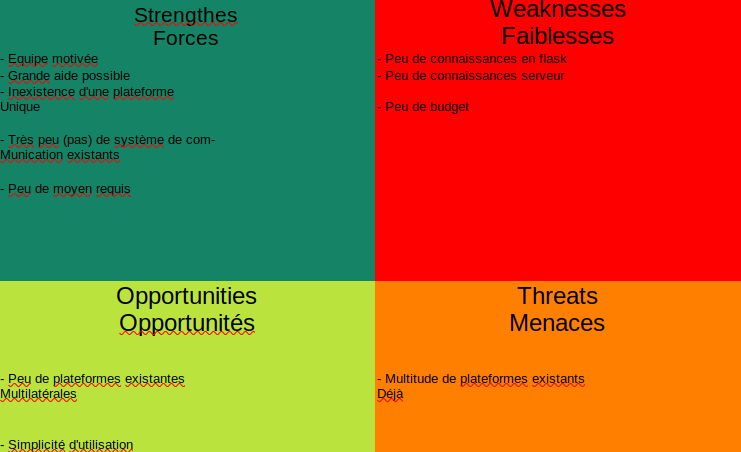
\includegraphics{SWOT}
